\documentclass[11pt, a4paper]{article}
\usepackage[utf8]{inputenc}
\usepackage[slovene]{babel}
\usepackage{amsmath}
\usepackage{amsfonts}
\usepackage{graphicx}
\usepackage{booktabs}
\usepackage{float}

\title{Domača naloga 3: Ničle Airyjeve funkcije}
\author{Anže Judež}
\date{\today}

\begin{document}

\maketitle

\section{Opis naloge}
Cilj naloge je bil poiskati ničle Airyjeve funkcije $Ai(x)$ na 10 decimalnih mest natančno\cite{textbook}. Airyjeva funkcija je definirana kot rešitev začetnega problema:
\begin{equation}
    Ai''(x) - x Ai(x) = 0, \quad Ai(0) = \frac{1}{3^{2/3} \Gamma(2/3)}, \quad Ai'(0) = -\frac{1}{3^{1/3} \Gamma(1/3)}.
\end{equation}
Za iskanje rešitve smo uporabili Magnusovo metodo reda 4 z iskanjem ničel s pomočjo bisekcije na podintervalih\cite{magnus1954, orel2004}.

\section{Matematično ozadje}
\subsection{Prevedba na sistem prvega reda}
Da bi lahko uporabili predlagano Magnusovo metodo, moramo diferencialno enačbo drugega reda prevesti na sistem prvega reda. Uvedemo novi spremenljivki $y_1(x) = Ai(x)$ in $y_2(x) = Ai'(x)$. Sistem se v matrični obliki zapiše kot:
\begin{equation}
    \begin{bmatrix} y_1'(x) \\ y_2'(x) \end{bmatrix} = \begin{bmatrix} 0 & 1 \\ x & 0 \end{bmatrix} \begin{bmatrix} y_1(x) \\ y_2(x) \end{bmatrix}
\end{equation}
od koder razberemo matriko sistema $A(x) = \begin{bmatrix} 0 & 1 \\ x & 0 \end{bmatrix}$.

\subsection{Magnusova metoda reda 4}
Reševanje sistema oblike $\mathbf{y}'(x) = A(x)\mathbf{y}(x)$ poteka iterativno. Nov približek na koraku $h$ se izračuna z matrično eksponentno funkcijo $\mathbf{y}_{k+1} = \exp(\sigma_{k+1})\mathbf{y}_k$, kjer je:
\begin{align}
    A_1 &= A\left(x_k + \left(\frac{1}{2} - \frac{\sqrt{3}}{6}\right)h\right), \\
    A_2 &= A\left(x_k + \left(\frac{1}{2} + \frac{\sqrt{3}}{6}\right)h\right), \\
    \sigma_{k+1} &= \frac{h}{2}(A_1 + A_2) - \frac{\sqrt{3}}{12}h^2 [A_1, A_2].
\end{align}
Izraz $[A_1, A_2] = A_1 A_2 - A_2 A_1$ predstavlja komutator matrik.

\section{Implementacija in iskanje ničel}
Sistem smo integrirali od $x = 0$ v negativno smer (ker ima funkcija ničle le za $x < 0$) s korakom $h = -0.01$. Med vsakim korakom smo preverili, ali je funkcija $y_1(x)$ spremenila predznak.

Če je bil zaznan prehod preko ničle na intervalu $[x_k, x_{k+1}]$, smo točno lokacijo ničle poiskali z modificirano **bisekcijo**. Bisekcija se ni izvajala na globalnem nivoju z reševanjem od začetka, temveč lokalno: delali smo deležne korake dolžine $t \cdot h$ (za $t \in [0, 1]$) iz že znane točke $x_k$ \cite{plestenjak2015}. Zaradi majhnosti koraka $h$ je taka lokalna Magnusova preslikava ekstremno natančna in ne kopiči globalne napake.

\section{Rezultati}
Z opisanim algoritmom smo poiskali ničle na intervalu $[0, -15]$. Rezultate smo preverili s pomočjo vgrajene funkcije \texttt{airyai} iz paketa \texttt{SpecialFunctions.jl}. Vrednost prave Airyjeve funkcije pri izračunanih ničlah je praktično enaka strojni ničli, kar dokazuje doseženo natančnost na več kot 10 decimalk.

\begin{table}[H]
    \centering
    \begin{tabular}{ccc}
        \toprule
        Zap. št. & Izračunana ničla ($x_n$) & Prava vrednost $Ai(x_n)$ \\
        \midrule
        1 & -2.33810741046 & $\sim 10^{-15}$ \\
        2 & -4.08794944413 & $\sim 10^{-15}$ \\
        3 & -5.52055982809 & $\sim 10^{-15}$ \\
        4 & -6.78670809007 & $\sim 10^{-14}$ \\
        5 & -7.94413358712 & $\sim 10^{-14}$ \\
        \bottomrule
    \end{tabular}
    \caption{Prvih pet ničel Airyjeve funkcije in ocena napake.}
\end{table}

\begin{figure}[H]
    \centering
    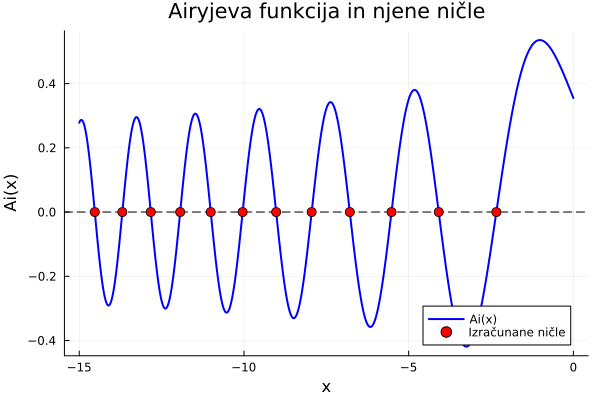
\includegraphics[width=0.8\textwidth]{airy_nicle.png}
    \caption{Graf Airyjeve funkcije z izračunanimi ničlami.}
\end{figure}

\section{Zaključek}
Prevedba začetnega problema drugega reda na sistem prvega reda omogoči učinkovito uporabo Magnusove metode. Metoda izkaže visoko stabilnost in natančnost. Kombinacija lokalne bisekcije in Magnusovega koraka reda 4 se izkaže kot izjemno robusten pristop, ki suvereno presega zahtevano relativno natančnost $10^{-10}$.

\begin{thebibliography}{9}

\bibitem{textbook} 
M. Vuk, \textit{Navodila za pripravo domačih nalog in opisi nalog (poglavja 17 in 18)}, Učbenik za numerične metode, 2026.

\bibitem{orel2004}
B. Orel, \textit{Osnove numerične matematike}, Fakulteta za računalništvo in informatiko, 2004.

\bibitem{plestenjak2015}
B. Plestenjak, \textit{Razširjen uvod v numerične metode}, DMFA - založništvo, 2015.

\bibitem{magnus1954}
W. Magnus, \textit{On the exponential solution of differential equations for a linear operator}, Communications on Pure and Applied Mathematics, 1954.

\bibitem{abramowitz}
M. Abramowitz, I. A. Stegun, \textit{Handbook of Mathematical Functions}, National Bureau of Standards, 1964.

\end{thebibliography}
\end{document}